\documentclass[fleqn,10pt]{olplainarticle}
% Use option lineno for line numbers 
\usepackage{caption}
\usepackage{subcaption}
\title{Machine Learning and Predictive Student Outcomes}

\author{Stacy Roberts}
\affil{robers23@utexas.edu}

\keywords{Machine Learning, Education, Student Outcomes, Student Success, Long-Term Success}

\begin{abstract}
Finding a solution to the problem of student success has long been a goal and a difficulty of education. Helping teachers, administrators, and support staff understand which students will benefit from additional intervention to achieve successful outcomes is assumed to increase the completion rate for all students. Being able to focus on what types of students are likely to need closer monitoring helps focus public school limited resources where they may see the highest return on investment. Accounting for co-variants outside of the school control is also necessary to understanding how best to serve the student population of a given school. This paper will focus on success in terms of standardized testing scores in Math, Reading, and Writing. Using various machine learning models, we attempt to demonstrate which pre-processing and models perform the best at predicting student success rates on subject testing.\end{abstract}

\begin{document}

\flushbottom
\maketitle
\thispagestyle{empty}

\section*{Introduction}

Predicting student outcomes is a necessary function of the public school system, which is tasked with maximizing the success of their entire student population. All schools are invested in the percentage of their students who graduate on time and go on to higher education or employment, as it is reflective of the success of the school itself. However, gaining access to student data is easier with public schools given the government mandates of public reporting they are required to follow. \citep{ecsa} This paper will focus on public school data.

There are many ideas of what types of students require more assistance to be successful in school. Focus is generally placed on socioeconomic background, race, gender, and parental education level. \citep{Bradley2022SESgap}  Time and again, higher socioeconomic areas have higher student achievement outcomes. This is true for both the high and low socioeconomic groups when the average status is higher for the area.  Higher SEG (Socioeconomic Groups) have many advantages, from stable homes and plentiful food to higher quality and more stable teaching and administrative staff at the schools which service them. \citep{HSEffectsLongTerm} This paper is not intending to check all possible differentials, but does note that it is difficult to separate all the co-variant factors which contribute to the success of a student population. Is it more important to have a stable, effective teaching staff or to provide a support system where all students have stability and enough food to eat? Ideal data sets for investigating this theory would involve students of equally matched SES with large differentials in staff quality, as well as students with same teachers but large differential in SES to attempt to isolate how important SES is for student success. Since families are generally uninterested in subjecting their children to be test subjects for educational theories which may impact their success, it is very difficult to find this type of data set.

Yet there are some pockets of students who outperform expectations based on background. \citep{YanGaiLowSEG} These students often have **need to finish this thought with other research**

This paper aims to utilize different Machine Learning models to see if we can train and fine tune a model to predict the students who are risk of failing standardized math, reading, and writing assessments based on available background information.
\section*{Research Background}
Efforts to improve student outcomes have had varying rates of success. There is no single path which guarantees that all students achieve high school graduation and beyond.  Instead, there is a continuous cycle of new research, new methods, new options to try to increase material retention, attendance, and ultimately, state testing scores.

Study after study has found that students who enter kindergarten behind their peers will struggle to make up the gap through their entire schooling. \citep{EdInequities} High quality and accessible pre-K, along with increasing availability of books at home have been shown to make significant improvements in preparing students for kindergarten. However, there are precious few resources for families on the lower and middle socioeconomic spectrum to access these trajectory changing elements for their children. \citep{cradleK} Providing more social safety nets such as paid parental leave, affordable child care, and more expanded and intensive services for families experiencing multiple adversities similar to every other developed nation would significantly improve the standing of children born into the more dire of situation.

Socioeconomic status also affects access to Twentieth century necessities like internet access and personal laptops. Given that nearly all school systems use online classrooms and school work, having access to a personal computer and internet at home is a requirement to be successful in school. However, personal computers come with a significant price tag and internet, even with income based discounts, is a monthly expense many families cannot afford.\citep{sesinternet} 

School systems focus on state testing scores as that is how they are ranked for public viewing. \citep{linnetal} These rankings then influence who chooses to buy homes within the district, which in turn influences the socioeconomic level of the population and the educational attainment and retention of the teaching, support, and admin staff attracted to said schools. The unfortunate side effect is that limited resources get reallocated to focus on preparation and support surrounding state testing, to the detriment of more holistic approaches to support the entire student. \citep{cradle}

\section*{Methods}
The data selected for analysis has anonymous student information. It includes columns for parental education, reduced/free lunch, whether they completed a test preparation course, along with gender and test scores for math, reading, and writing assessments. There is enough information to make an educated guess as to the socioeconomic level of each student. I based the socioeconomic level on parental education and whether the student was on reduced/free lunch plan.  Many studies base it on the mother's level of education, but this data set doesn't have that sort of granularity. \citep{maternaleducation}

I began my training by doing pre-processing of the original data. I wanted to see the data analysis correlating the parent's education level with the passing rates of their children. I kept each of the individual standardized testing areas separate to see if there were different correlations for the different subjects. Graphs demonstrated a small difference in outcomes between the subject areas, but it was more noticeable the variability of the pass rate within each group than how many of the students of each group passed.

\begin{figure}[h!]
    \centering
    \caption{Correlations of Parent Education to Student Subject Scores}
    \begin{subfigure}{0.3\textwidth}
    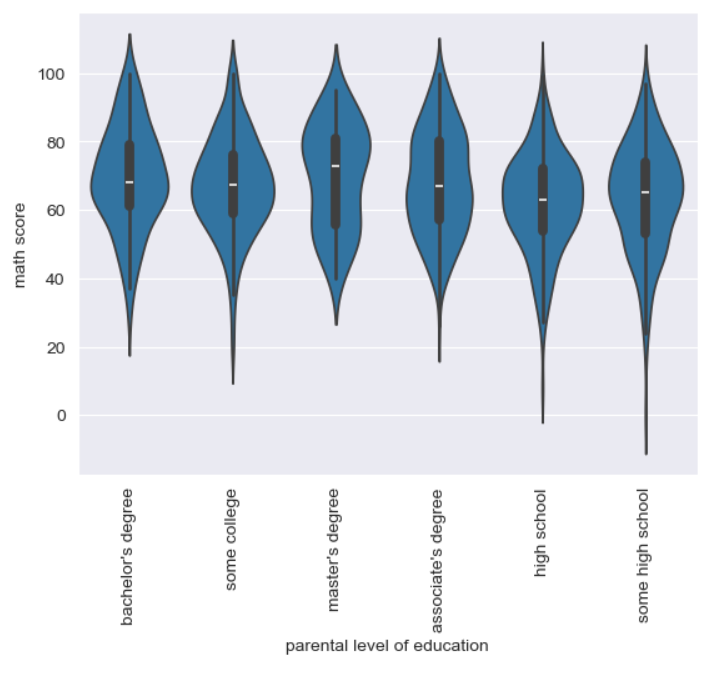
\includegraphics[width=\linewidth]{MathVsParent.png}
    \caption{Correlation of Math Scores}
    \label{fig:1.a}
    \end{subfigure}
    \begin{subfigure}{0.3\textwidth}
    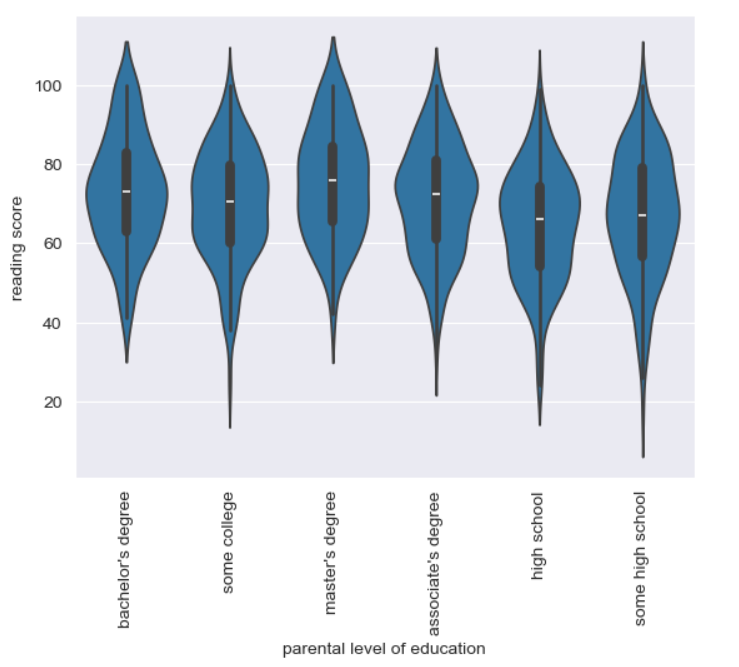
\includegraphics[width=\linewidth]{ReadingVsParent.png}
    \caption{Correlation of Reading Scores}
    \label{fig:1.b}
    \end{subfigure}
    \begin{subfigure}{0.3\textwidth}
    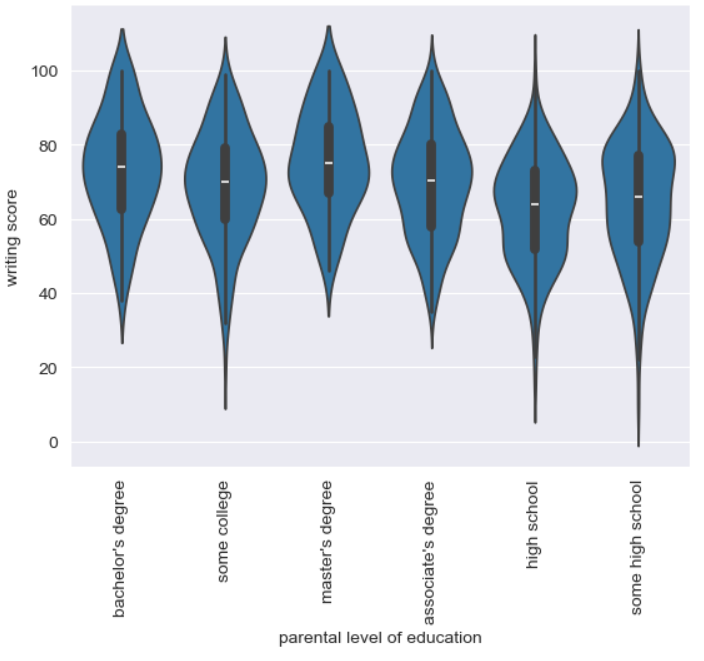
\includegraphics[width=\linewidth]{WritingVsParent.png}
    \caption{Correlation of Writing Scores}
    \label{fig:1.c}
    \end{subfigure}
\end{figure}

As noted here in the Math scores, while the students of all parental education levels were able to attain a similar top end score, the variability of the plot indicates a higher mean the more education the parents were able to obtain.  Students of parents with a Master's degree had the highest mean math score, but there isn't a big difference in the mean for the other categories.  The most noticeable difference between the categories is the lowest score rate. The lower the education level of the parents, the lower the lowest scores of the students.  Clearly there is some correlation, but not as strong of one as might be expected based on the volume of literature around SES and student success.

Similar to the Math score graph, the Writing scores show variability relative to parental education level.  It is a bit more noticeable that those whose parents only achieved at most high school level of education had a lower mean and bottom end scores in writing. It would appear that within this dataset, the influence of parent's education is more noticeable in writing ability.

\section*{Results and Analysis}
\section*{Conclusion}
\section*{Glossary}
Given there are some terms which come up over and over, I will provide the intended definitions to the most prevalent ones here.

\begin{description}
\item[SES] Socioeconomic Status. Defined as low, medium, or high, it relates to a family's wealth and income, educational attainment, occupational prestige, and perceived social status and social class.\citep{sesdef}
\item[SEG] Socioeconomic Groups. Defined as the people belonging within the same Socioeconomic status
\end{description}

\section*{Some \LaTeX{} Examples}
\label{sec:examples}

Use section and subsection commands to organize your document. \LaTeX{} handles all the formatting and numbering automatically. Use ref and label commands for cross-references.

\subsection*{Figures and Tables}

Use the table and tabular commands for basic tables --- see Table~\ref{tab:widgets}, for example. You can upload a figure (JPEG, PNG or PDF) using the project menu. To include it in your document, use the include graphics command as in the code for Figure~\ref{fig:view} below.

\begin{figure}[ht]
\centering
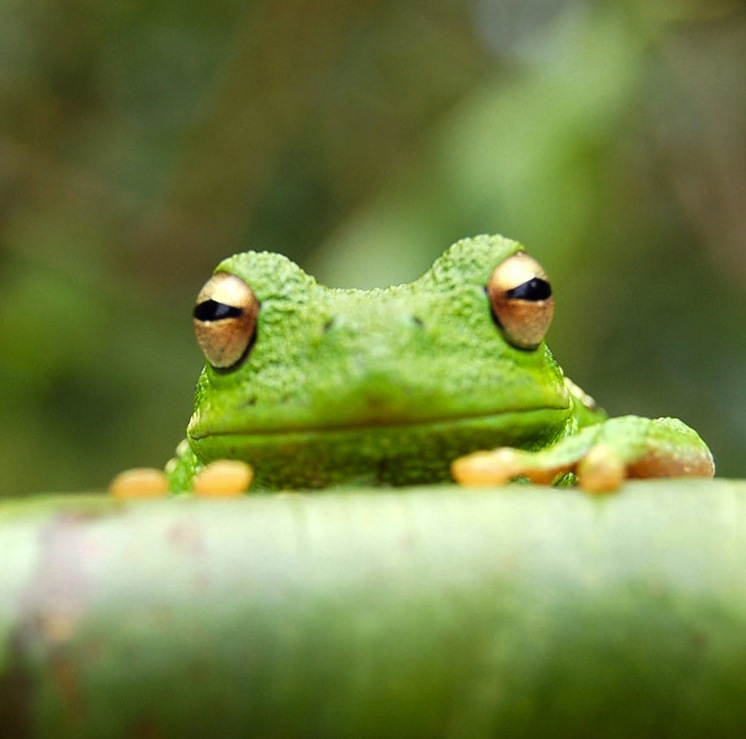
\includegraphics[width=0.7\linewidth]{frog}
\caption{An example image of a frog.}
\label{fig:view}
\end{figure}

\begin{table}[ht]
\centering
\begin{tabular}{l|r}
Item & Quantity \\\hline
Candles & 4 \\
Fork handles & ?  
\end{tabular}
\caption{\label{tab:widgets}An example table.}
\end{table}

\subsection*{Citations}

LaTeX formats citations and references automatically using the bibliography records in your .bib file, which you can edit via the project menu. Use the cite command for an inline citation, like \cite{Bradley2022SESgap}, and the citep command for a citation in parentheses \citep{Bradley2022SESgap}.

\subsection*{Mathematics}

\LaTeX{} is great at typesetting mathematics. Let $X_1, X_2, \ldots, X_n$ be a sequence of independent and identically distributed random variables with $\text{E}[X_i] = \mu$ and $\text{Var}[X_i] = \sigma^2 < \infty$, and let
$$S_n = \frac{X_1 + X_2 + \cdots + X_n}{n}
      = \frac{1}{n}\sum_{i}^{n} X_i$$
denote their mean. Then as $n$ approaches infinity, the random variables $\sqrt{n}(S_n - \mu)$ converge in distribution to a normal $\mathcal{N}(0, \sigma^2)$.

\subsection*{Lists}

You can make lists with automatic numbering \dots

\begin{enumerate}[noitemsep] 
\item Like this,
\item and like this.
\end{enumerate}
\dots or bullet points \dots
\begin{itemize}[noitemsep] 
\item Like this,
\item and like this.
\end{itemize}
\dots or with words and descriptions \dots
\begin{description}
\item[Word] Definition
\item[Concept] Explanation
\item[Idea] Text
\end{description}


\bibliographystyle{apa}
\bibliography{./sample.bib}

\end{document}